\section{Human Handover Analysis}

\subsection{Experimental Scenario}
- talk about the necessity of performing this HHI experiments 

- explain the HHI experiment

- present an image

\subsection{Handover Analysis}

- analysis the data distance/velocity (inverse time of flight)

- analysis the data time/velocity

- mention that in the results we present two other datasets (QMUL, IST)

\subsection{Discussion}

- resume what you see from the data analysis of the human wrist

    \begin{figure}[t]
      \centering
      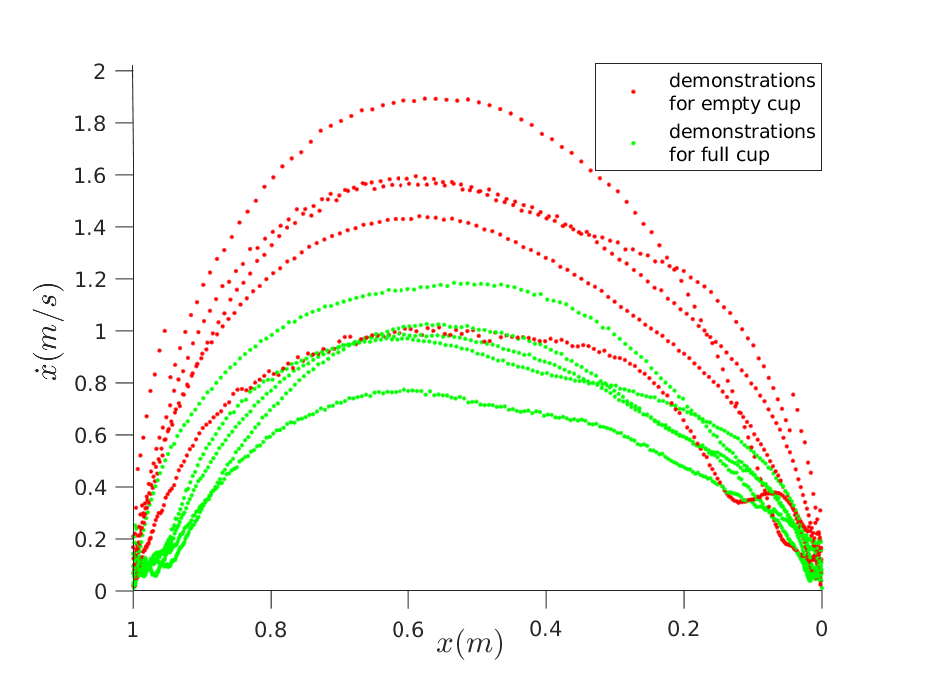
\includegraphics[width = 0.48\textwidth]{Images/vel_distance_plot.eps}
      \caption{Add legend} 
      \label{fig:vel_distance}
	\end{figure}
	
	
    \begin{figure}[t]
      \centering
      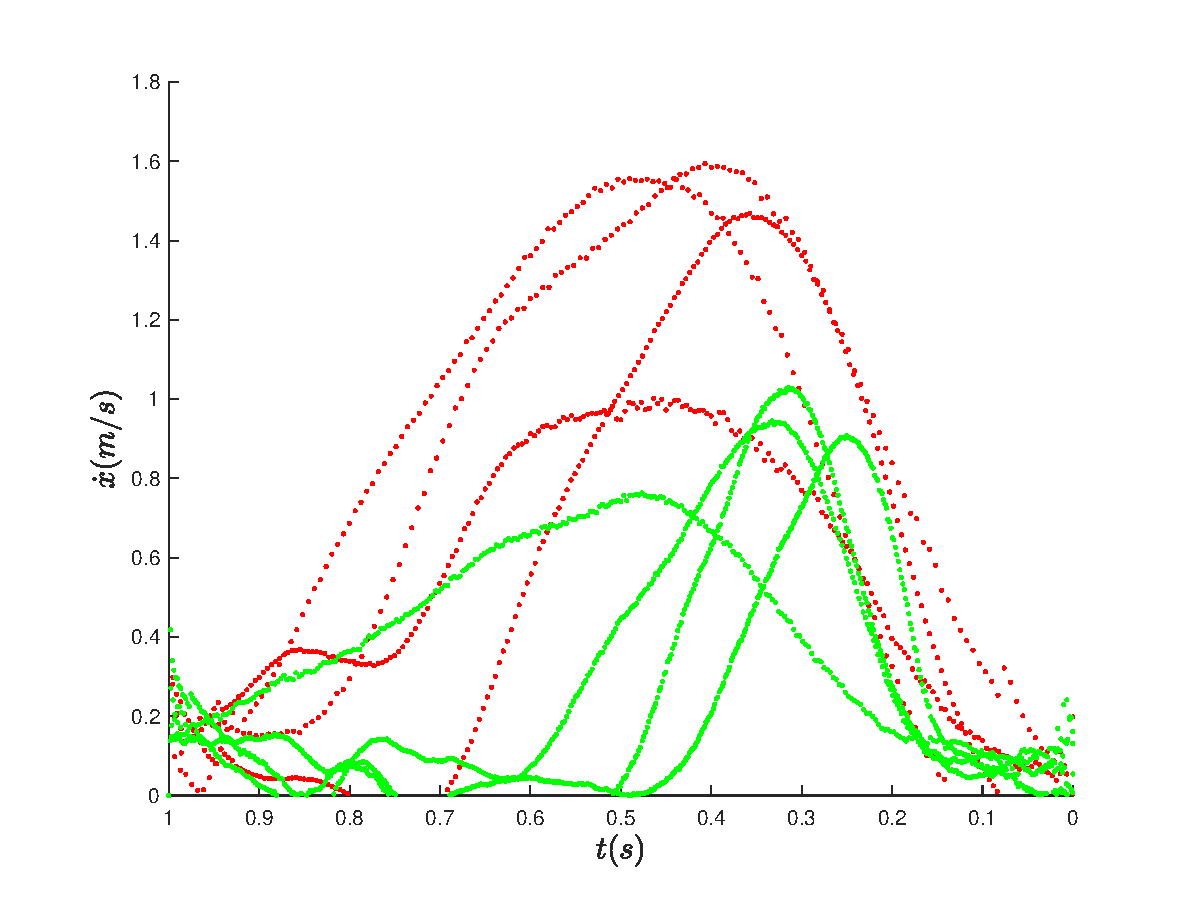
\includegraphics[width = 0.48\textwidth]{Images/vel_time_plot.eps}
      \caption{Add legend} 
      \label{fig:vel_time}
	\end{figure}
	